% This file was created by tikzplotlib v0.9.1.
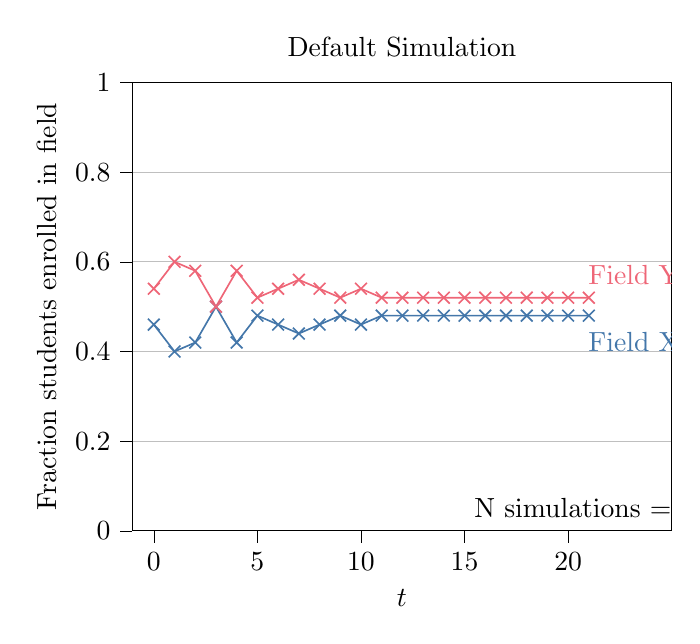
\begin{tikzpicture}

\definecolor{color0}{rgb}{0.266666666666667,0.466666666666667,0.666666666666667}
\definecolor{color1}{rgb}{0.933333333333333,0.4,0.466666666666667}

\begin{axis}[
height=207pt,
tick align=outside,
tick pos=left,
title={Default Simulation},
width=240pt,
x grid style={white!69.0196078431373!black},
xlabel={\(\displaystyle t\)},
xmin=-1.05, xmax=25,
xtick style={color=black},
xtick={0,5,10,15,20},
xticklabels={\(\displaystyle 0\),\(\displaystyle 5\),\(\displaystyle 10\),\(\displaystyle 15\),\(\displaystyle 20\)},
ylabel={Fraction students enrolled in field},
ymajorgrids,
ymin=0, ymax=1,
ytick style={color=black}
]
\addplot [semithick, color0, mark=x, mark size=3, mark options={solid}]
table {%
0 0.46
1 0.4
2 0.42
3 0.5
4 0.42
5 0.48
6 0.46
7 0.44
8 0.46
9 0.48
10 0.46
11 0.48
12 0.48
13 0.48
14 0.48
15 0.48
16 0.48
17 0.48
18 0.48
19 0.48
20 0.48
21 0.48
};
\addplot [semithick, color1, mark=x, mark size=3, mark options={solid}]
table {%
0 0.54
1 0.6
2 0.58
3 0.5
4 0.58
5 0.52
6 0.54
7 0.56
8 0.54
9 0.52
10 0.54
11 0.52
12 0.52
13 0.52
14 0.52
15 0.52
16 0.52
17 0.52
18 0.52
19 0.52
20 0.52
21 0.52
};
\draw (axis cs:20.5,0.4) node[
  anchor=base west,
  text=color0,
  rotate=0.0
]{Field X};
\draw (axis cs:20.5,0.55) node[
  anchor=base west,
  text=color1,
  rotate=0.0
]{Field Y};
\draw (axis cs:15,0.03) node[
  anchor=base west,
  text=black,
  rotate=0.0
]{N simulations = 50};
\end{axis}

\end{tikzpicture}
